\documentclass[11pt,letterpaper]{article}
\usepackage[margin=1in]{geometry}
\usepackage{graphicx}
\usepackage{hyperref}
\usepackage{booktabs}
\usepackage{xcolor}
\usepackage{listings}
\usepackage{textcomp}
\usepackage{url}

\graphicspath{{figures/}}

\lstset{
  basicstyle=\ttfamily\small,
  frame=single,
  breaklines=true,
  columns=fullflexible,
  backgroundcolor=\color{gray!8}
}

\hypersetup{colorlinks=true, urlcolor=blue, linkcolor=blue}

\title{meteoearth User and Developer Manual\\[2pt]
       \large An interactive globe for live NOAA GFS weather}
\author{Paul Fishwick and Claude Code}
\date{June 2026}

\begin{document}

\maketitle
\tableofcontents
\newpage

\section{Introduction}

meteoearth is a single-page, browser-based globe that visualizes live weather
from the NOAA Global Forecast System (GFS). It renders animated wind particles,
switchable scalar overlays (temperature, humidity, pressure, cloud, precipitable
water), labeled high- and low-pressure centers, and point readouts on hover and
right-click. It is modeled on the spirit of \texttt{earth.nullschool.net} but
built on deck.gl's \texttt{GlobeView} with the WeatherLayers GL community
edition, and backed by a small Python pipeline that turns GRIB2 model output
into compact PNG textures.

As shown in Figure~\ref{fig:overview}, the workspace is a draggable, zoomable
globe. Wind flows as luminous particle trails; a control panel sits at lower
left; the run timestamp is shown at upper left; and blue \textbf{L} / red
\textbf{H} glyphs mark the centers of the cyclones and anticyclones.

\begin{figure}[h]
\centering
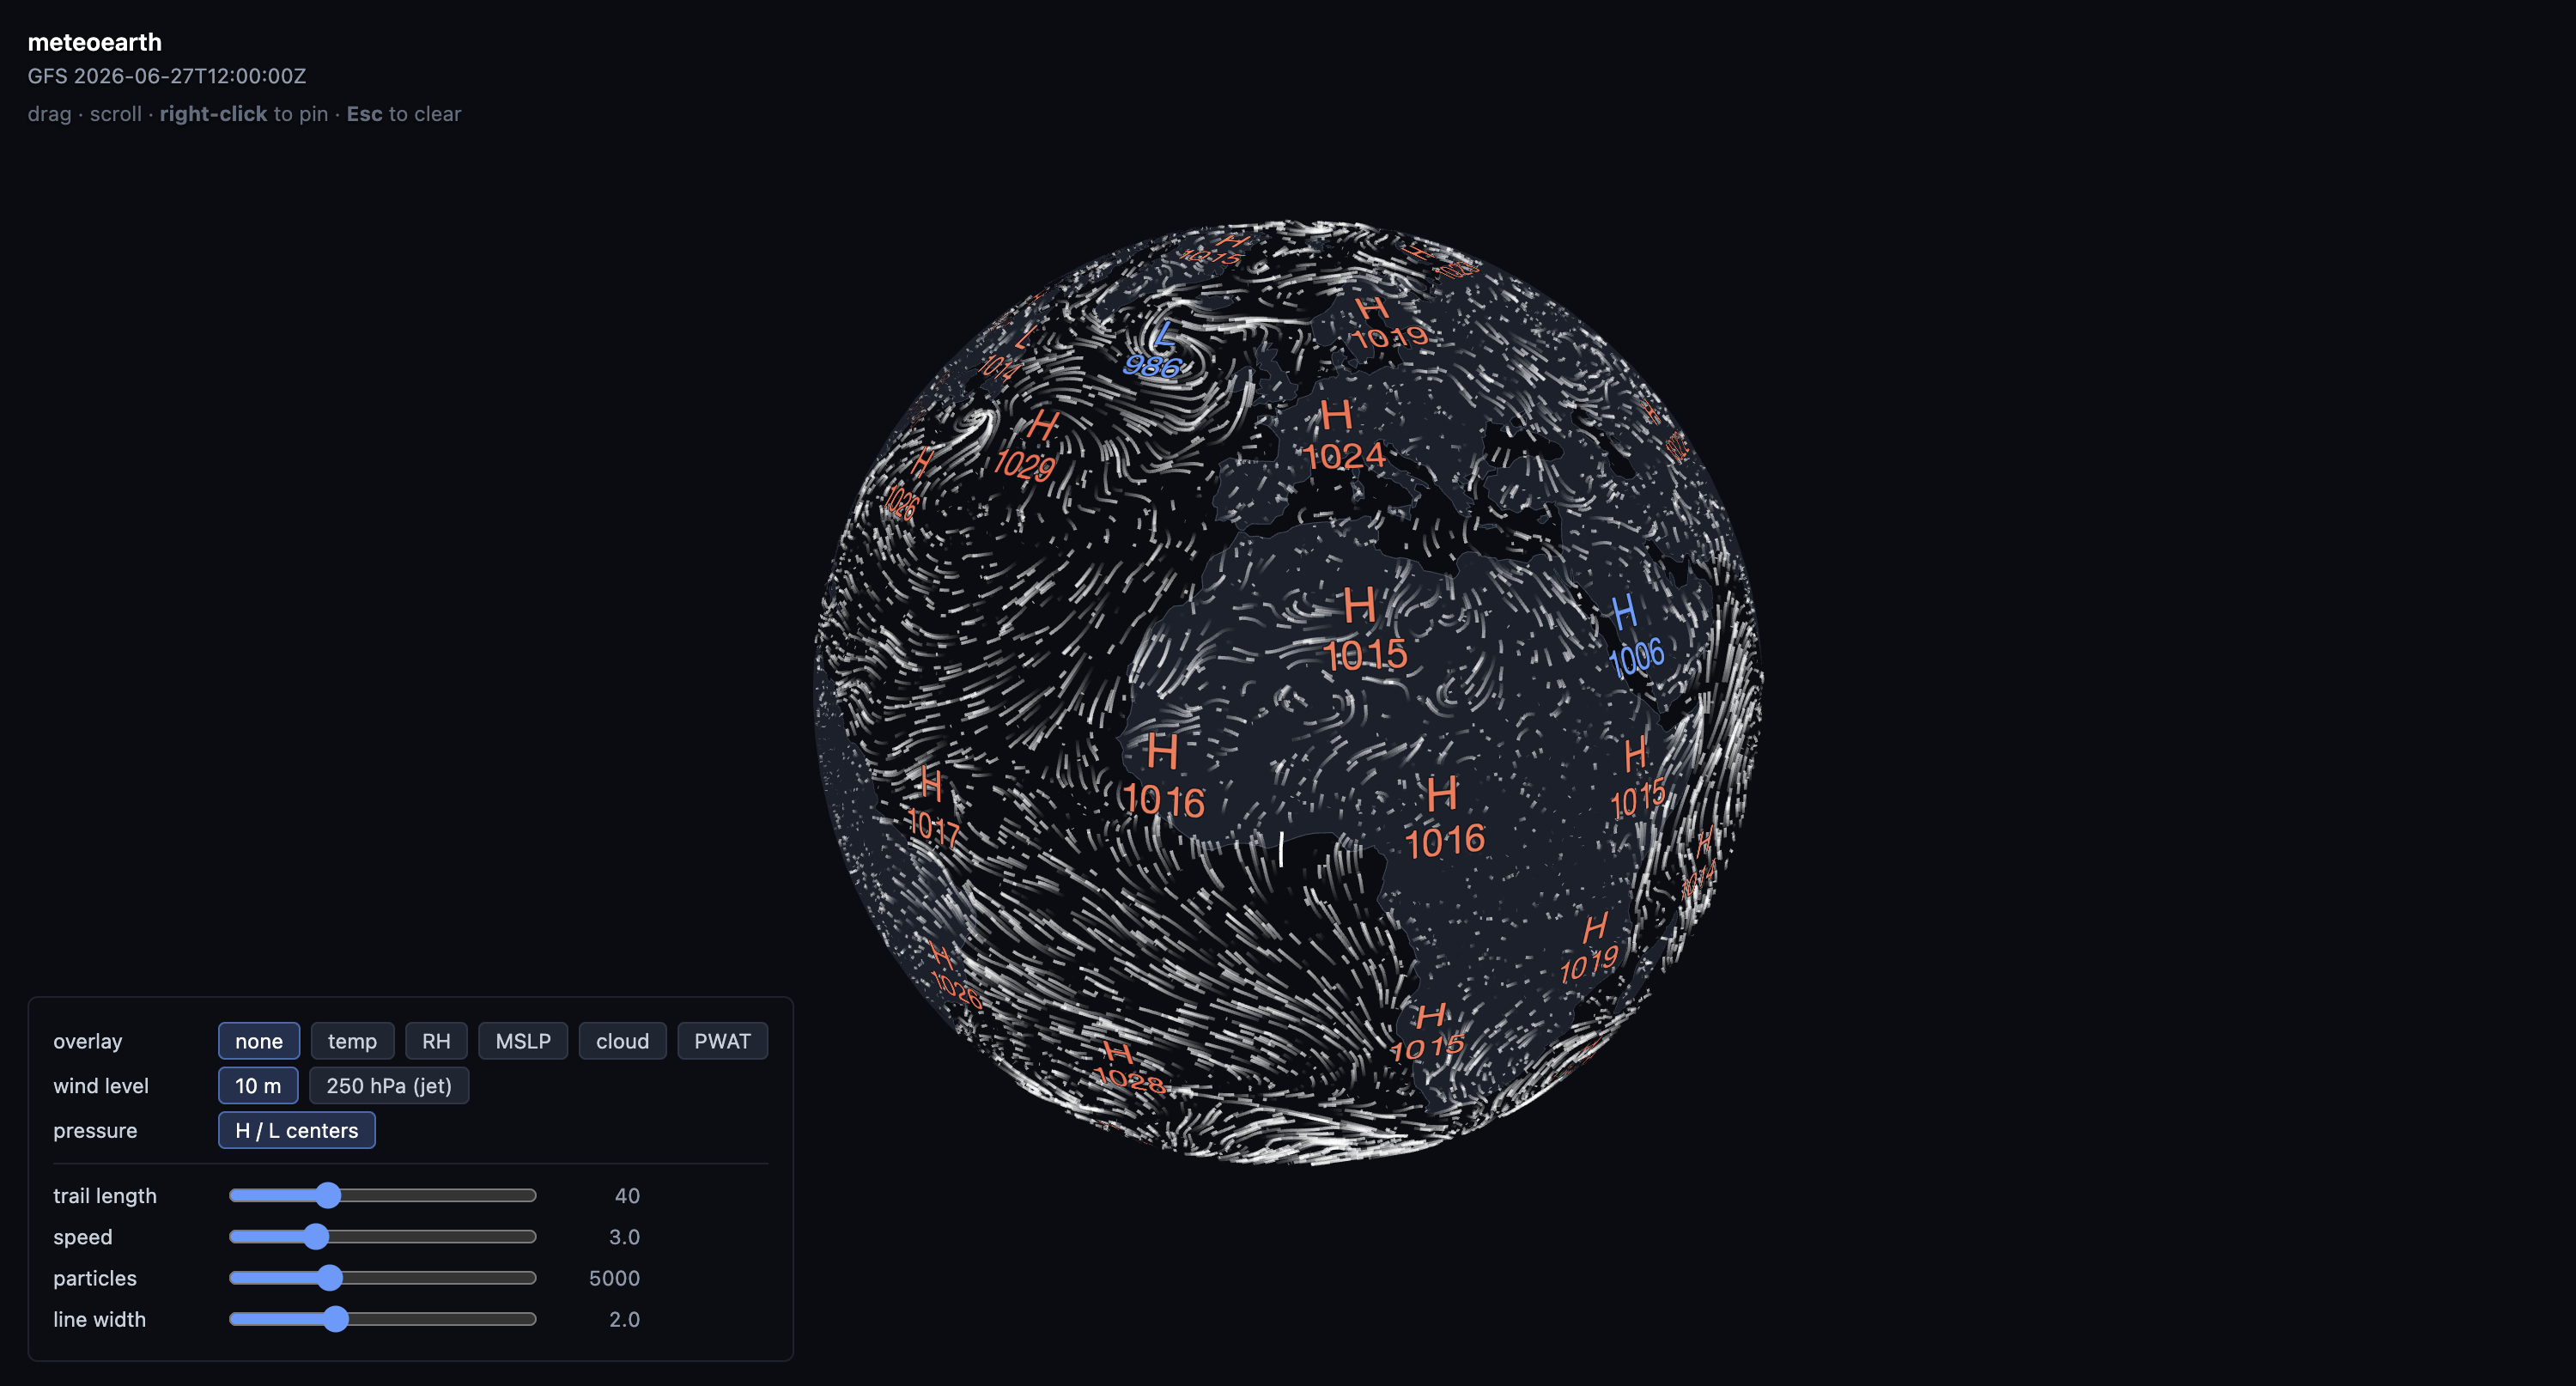
\includegraphics[width=0.92\textwidth]{fig_overview.png}
\caption{The meteoearth globe as it loads: 10\,m wind particles over open ocean
and land, with high/low pressure centers labeled. The control panel (lower left)
selects overlays, wind level, and particle appearance.}
\label{fig:overview}
\end{figure}

\subsection{Design Goals}
\begin{itemize}
  \item \textbf{Live data.} A single \texttt{refresh-data.sh} pulls the latest
        GFS cycle and rebuilds every layer.
  \item \textbf{No build step.} The frontend is one HTML file plus one JS module,
        loading deck.gl and WeatherLayers from a CDN.
  \item \textbf{Compact transport.} Each variable is packed into a PNG and a
        small JSON of metadata, sampled client-side for instant readouts.
  \item \textbf{Reproducible provenance.} Every layer traces back to an explicit
        GFS field and level (\S\ref{sec:data}).
\end{itemize}

\section{Installation and Setup}

meteoearth has been developed and tested on macOS (Apple Silicon). Dependencies:
\begin{itemize}
  \item Python 3.10+ with a local \texttt{venv}
  \item A modern Chromium-based browser
  \item (for figures/tests) Selenium with a matching ChromeDriver
\end{itemize}

The repository root contains the operational scripts:
\begin{lstlisting}
./refresh-data.sh   # pull latest GFS cycle + rebuild data/ (~30 s)
./start             # serve http://localhost:5862 and open the globe
./stop              # stop the local server
\end{lstlisting}

\texttt{./start} launches a static HTTP server on port 5862 and opens
\url{http://localhost:5862/frontend/index.html}. Run \texttt{./refresh-data.sh}
at least once first so the \texttt{data/} directory is populated.

\section{Data and Provenance}
\label{sec:data}

Every layer in meteoearth comes from one place: the NOAA NCEP Global Forecast
System, retrieved as GRIB2 \emph{subsets} from the NOMADS filter endpoint. The
download is driven entirely by \texttt{pipeline/fetch\_gfs.py}, which reads the
variable registry in \texttt{pipeline/variables.py} and requests only the exact
fields and levels needed (each subset is a few hundred KB rather than the full
multi-hundred-MB GRIB file). The pipeline discovers the most recent published
cycle (00/06/12/18\,UTC, padded for publication lag) and downloads the analysis
hour (f000) at 0.5\textdegree{} global resolution.

Table~\ref{tab:data} is the complete inventory of ingested data. It is not
hand-written: it is generated by \texttt{docs/gen\_data\_sources.py}, which
imports the same registry the downloader uses, so the manual cannot drift from
what is actually fetched.

% AUTO-GENERATED by docs/gen_data_sources.py -- do not edit by hand.
\begin{table}[h]
\centering
\footnotesize
\setlength{\tabcolsep}{5pt}
\begin{tabular}{@{}l p{3.0cm} l c l l@{}}
\toprule
\textbf{Source} & \textbf{Model} & \textbf{Res.} & \textbf{Vars} & \textbf{Steps} & \textbf{Cycle} \\
\midrule
  \texttt{gfs} & NOAA GFS & 0.5\textdegree{} & 10 & f000--f048/3h & \texttt{2026-06-28T18:00:00Z} \\
  \texttt{ecmwf} & ECMWF IFS & 0.25\textdegree{} & 7 & f000--f048/3h & \texttt{2026-06-28T06:00:00Z} \\
  \texttt{gem} & ECCC GEM & 0.15\textdegree{} & 8 & f000--f048/3h & \texttt{2026-06-28T12:00:00Z} \\
\bottomrule
\end{tabular}
\caption{The global forecast models meteoearth ingests, generated from
\texttt{data/index.json} by \texttt{docs/gen\_data\_sources.py}. Each model
is fetched independently from its own provider (NOMADS, ECMWF open data, and the
MSC hpfx server) at its native resolution, for the analysis hour through a
two-day forecast.}
\label{tab:sources}
\end{table}

\begin{table}[h]
\centering
\footnotesize
\setlength{\tabcolsep}{6pt}
\begin{tabular}{@{}l p{3.2cm} l c c c@{}}
\toprule
\textbf{Layer} & \textbf{Quantity} & \textbf{Units} & \textbf{gfs} & \textbf{ecmwf} & \textbf{gem} \\
\midrule
  \texttt{wind\_10m} & 10 m wind & m/s & \checkmark & \checkmark & \checkmark \\
  \texttt{wind\_250mb} & 250 hPa wind (jet stream) & m/s & \checkmark & \checkmark & \checkmark \\
  \texttt{tmp\_2m} & 2 m temperature & \textdegree{}C & \checkmark & \checkmark & \checkmark \\
  \texttt{rh\_2m} & 2 m relative humidity & \% & \checkmark & -- & \checkmark \\
  \texttt{mslp} & Mean sea-level pressure & hPa & \checkmark & \checkmark & \checkmark \\
  \texttt{cloud\_cover} & Total cloud cover & \% & \checkmark & \checkmark & \checkmark \\
  \texttt{pwat} & Total precipitable water & kg/m\textsuperscript{2} & \checkmark & \checkmark & -- \\
  \texttt{gust} & Wind gusts & m/s & \checkmark & \checkmark & \checkmark \\
  \texttt{prate} & Precipitation rate & mm/h & \checkmark & -- & -- \\
  \texttt{cape} & CAPE (thunderstorm potential) & J/kg & \checkmark & -- & \checkmark \\
\bottomrule
\end{tabular}
\caption{Canonical layers and which models provide each one. Where a model does
not publish a field (e.g.\ ECMWF open data has no plain CAPE or instantaneous
precipitation, GEM no precipitable water), the corresponding overlay is greyed
out when that model is selected.}
\label{tab:coverage}
\end{table}


After download, \texttt{pipeline/decode.py} reads each GRIB2 file with
\texttt{cfgrib}, applies any unit transform (e.g.\ K\,$\to$\,\textdegree{}C,
Pa\,$\to$\,hPa), and \texttt{pipeline/encode.py} linearly packs the values into
an 8-bit PNG (the R/G channels carry $u$/$v$ for vector fields; a single channel
carries scalars) alongside a JSON of bounds, the encode range, run/valid times,
and a color palette. The provenance chain for any layer is therefore:
\begin{center}
NOMADS GFS subset $\rightarrow$ \texttt{decode.py} $\rightarrow$
\texttt{encode.py} $\rightarrow$ \texttt{data/<layer>.png} + \texttt{.json}
$\rightarrow$ frontend.
\end{center}

\section{Interface Tour}

\subsection{Globe Navigation}
Drag to rotate, scroll to zoom. The view is a true 3-D globe, so layers wrap
seamlessly across the date line and converge correctly at the poles.

\subsection{Control Panel}
The lower-left panel (visible in every figure) has three button rows and four
sliders:
\begin{itemize}
  \item \textbf{overlay} --- choose the scalar layer painted on the globe
        (\texttt{none}, temp, RH, MSLP, cloud, PWAT). Mutually exclusive.
  \item \textbf{wind level} --- switch the particle field between 10\,m surface
        wind and the 250\,hPa jet stream.
  \item \textbf{pressure} --- the \texttt{H\,/\,L centers} toggle (on by
        default); see \S\ref{sec:highlow}.
  \item \textbf{sliders} --- trail length, speed, particle count, and line width
        for the wind animation.
\end{itemize}

\subsection{Hover and Pin Readouts}
Moving the cursor over the globe shows a near-cursor badge with the latitude and
longitude and every variable sampled at that point --- including the mean
sea-level pressure. Right-clicking \emph{pins} a point: a persistent panel
(Figure~\ref{fig:pin}) holds the readout until dismissed with the \texttt{\(\times\)}
button or the \texttt{Esc} key.

\begin{figure}[h]
\centering
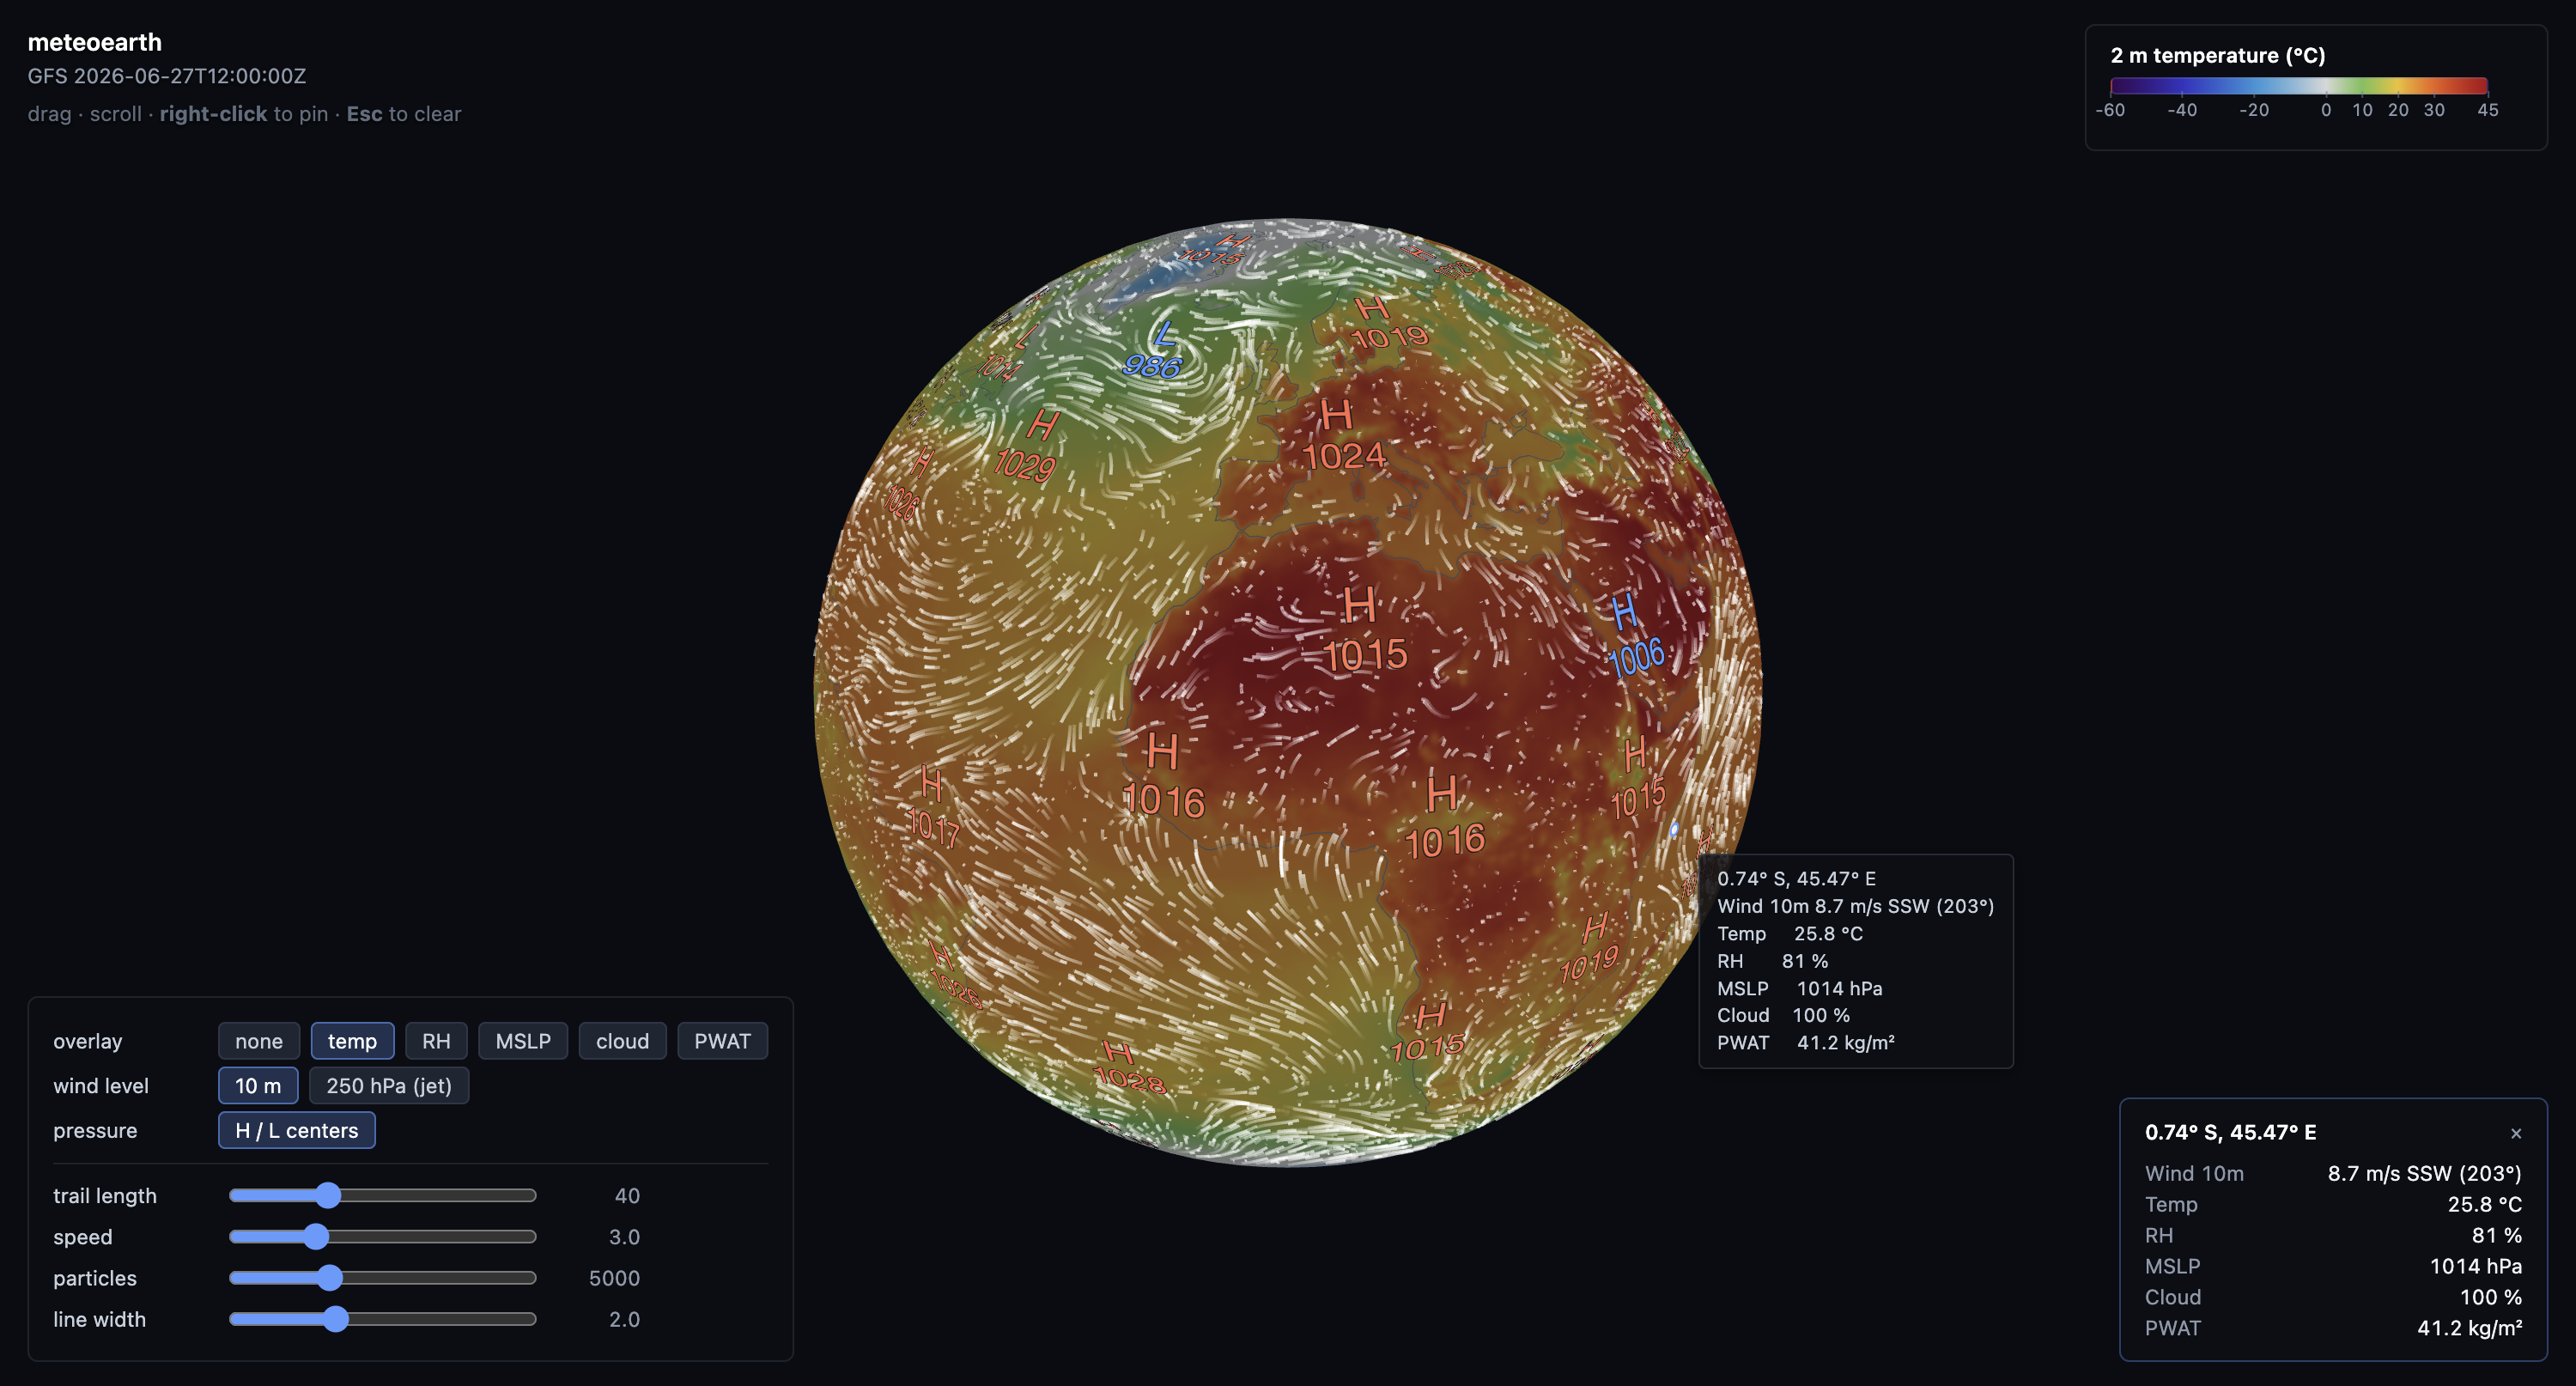
\includegraphics[width=0.92\textwidth]{fig_pin.png}
\caption{A pinned point over the temperature overlay. The right-hand panel keeps
the full multi-variable readout (wind, temperature, humidity, pressure, cloud,
precipitable water) for the marked location.}
\label{fig:pin}
\end{figure}

\section{Scalar Overlays}

Selecting an overlay paints a GFS field on the globe with a per-variable palette
and shows a matching colorbar legend at upper right. Two representative overlays
are shown here. Temperature (Figure~\ref{fig:temp}) runs from deep violet
(coldest) to dark red (hottest). Total precipitable water
(Figure~\ref{fig:pwat}) reveals atmospheric rivers as bright moisture plumes.
The cloud-cover overlay (not shown) renders a grayscale, satellite-like field,
and MSLP is shown later with the pressure centers (Figure~\ref{fig:highlow}).

\begin{figure}[h]
\centering
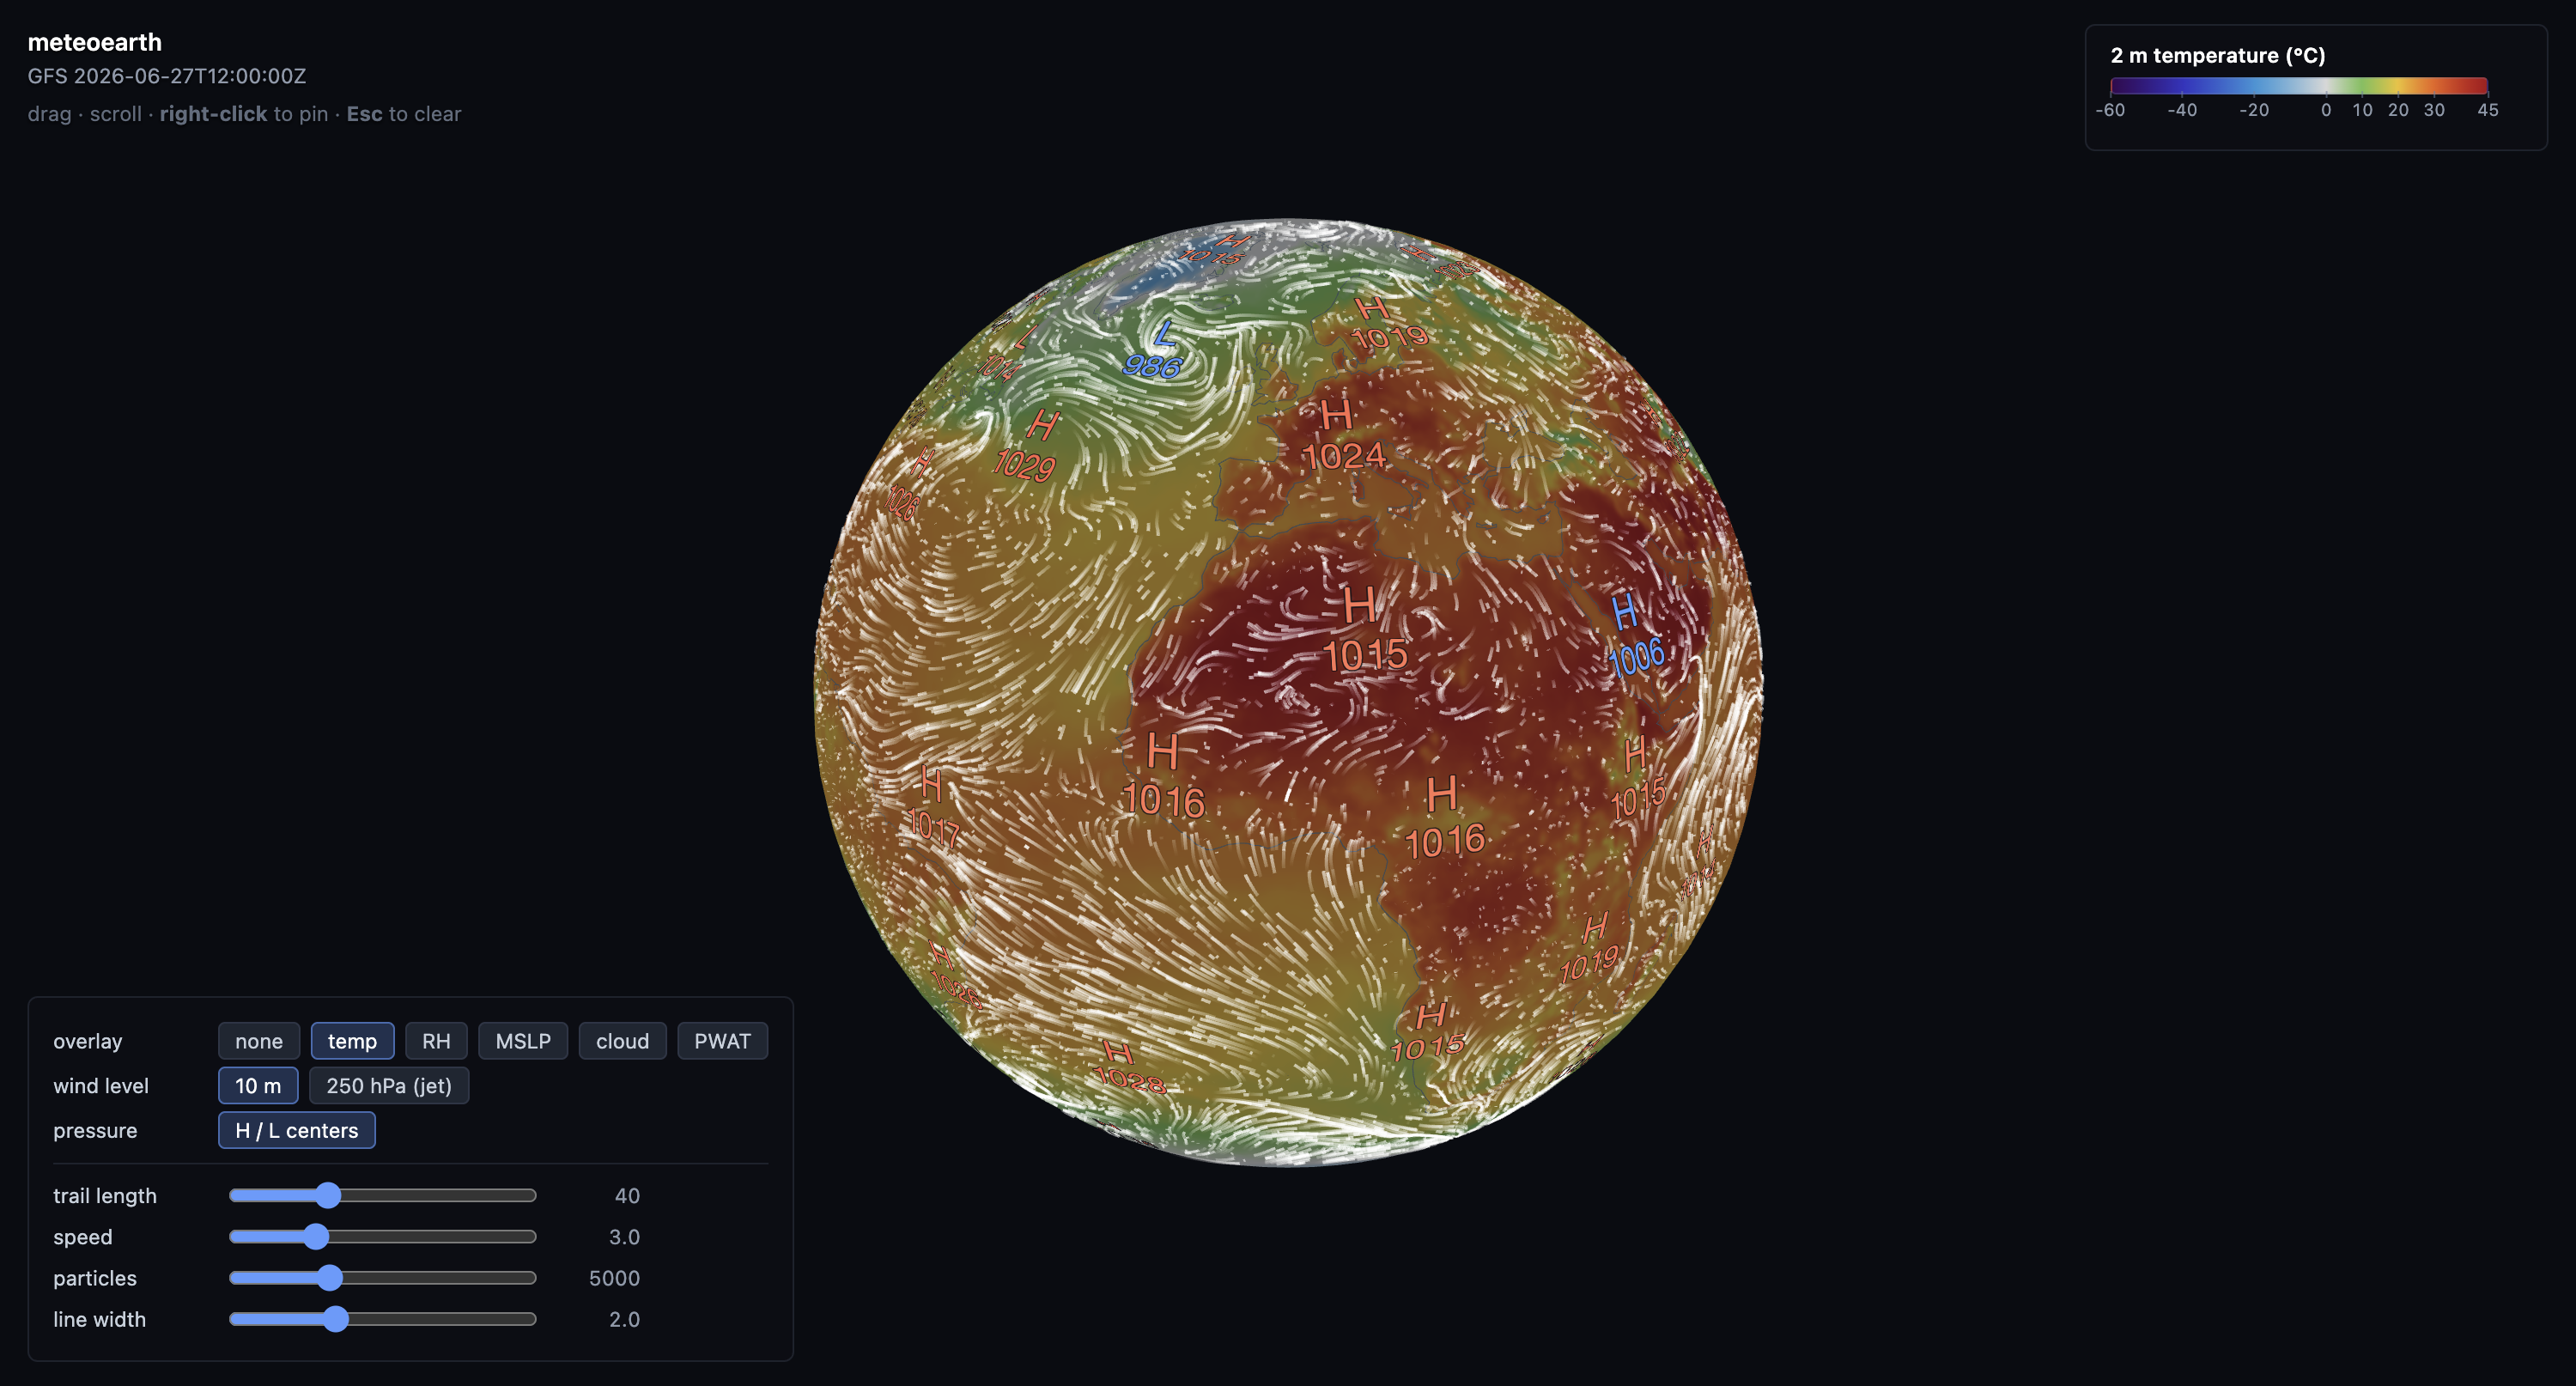
\includegraphics[width=0.92\textwidth]{fig_temp.png}
\caption{2\,m temperature overlay. The legend at upper right is built directly
from the layer's palette stops.}
\label{fig:temp}
\end{figure}

\begin{figure}[h]
\centering
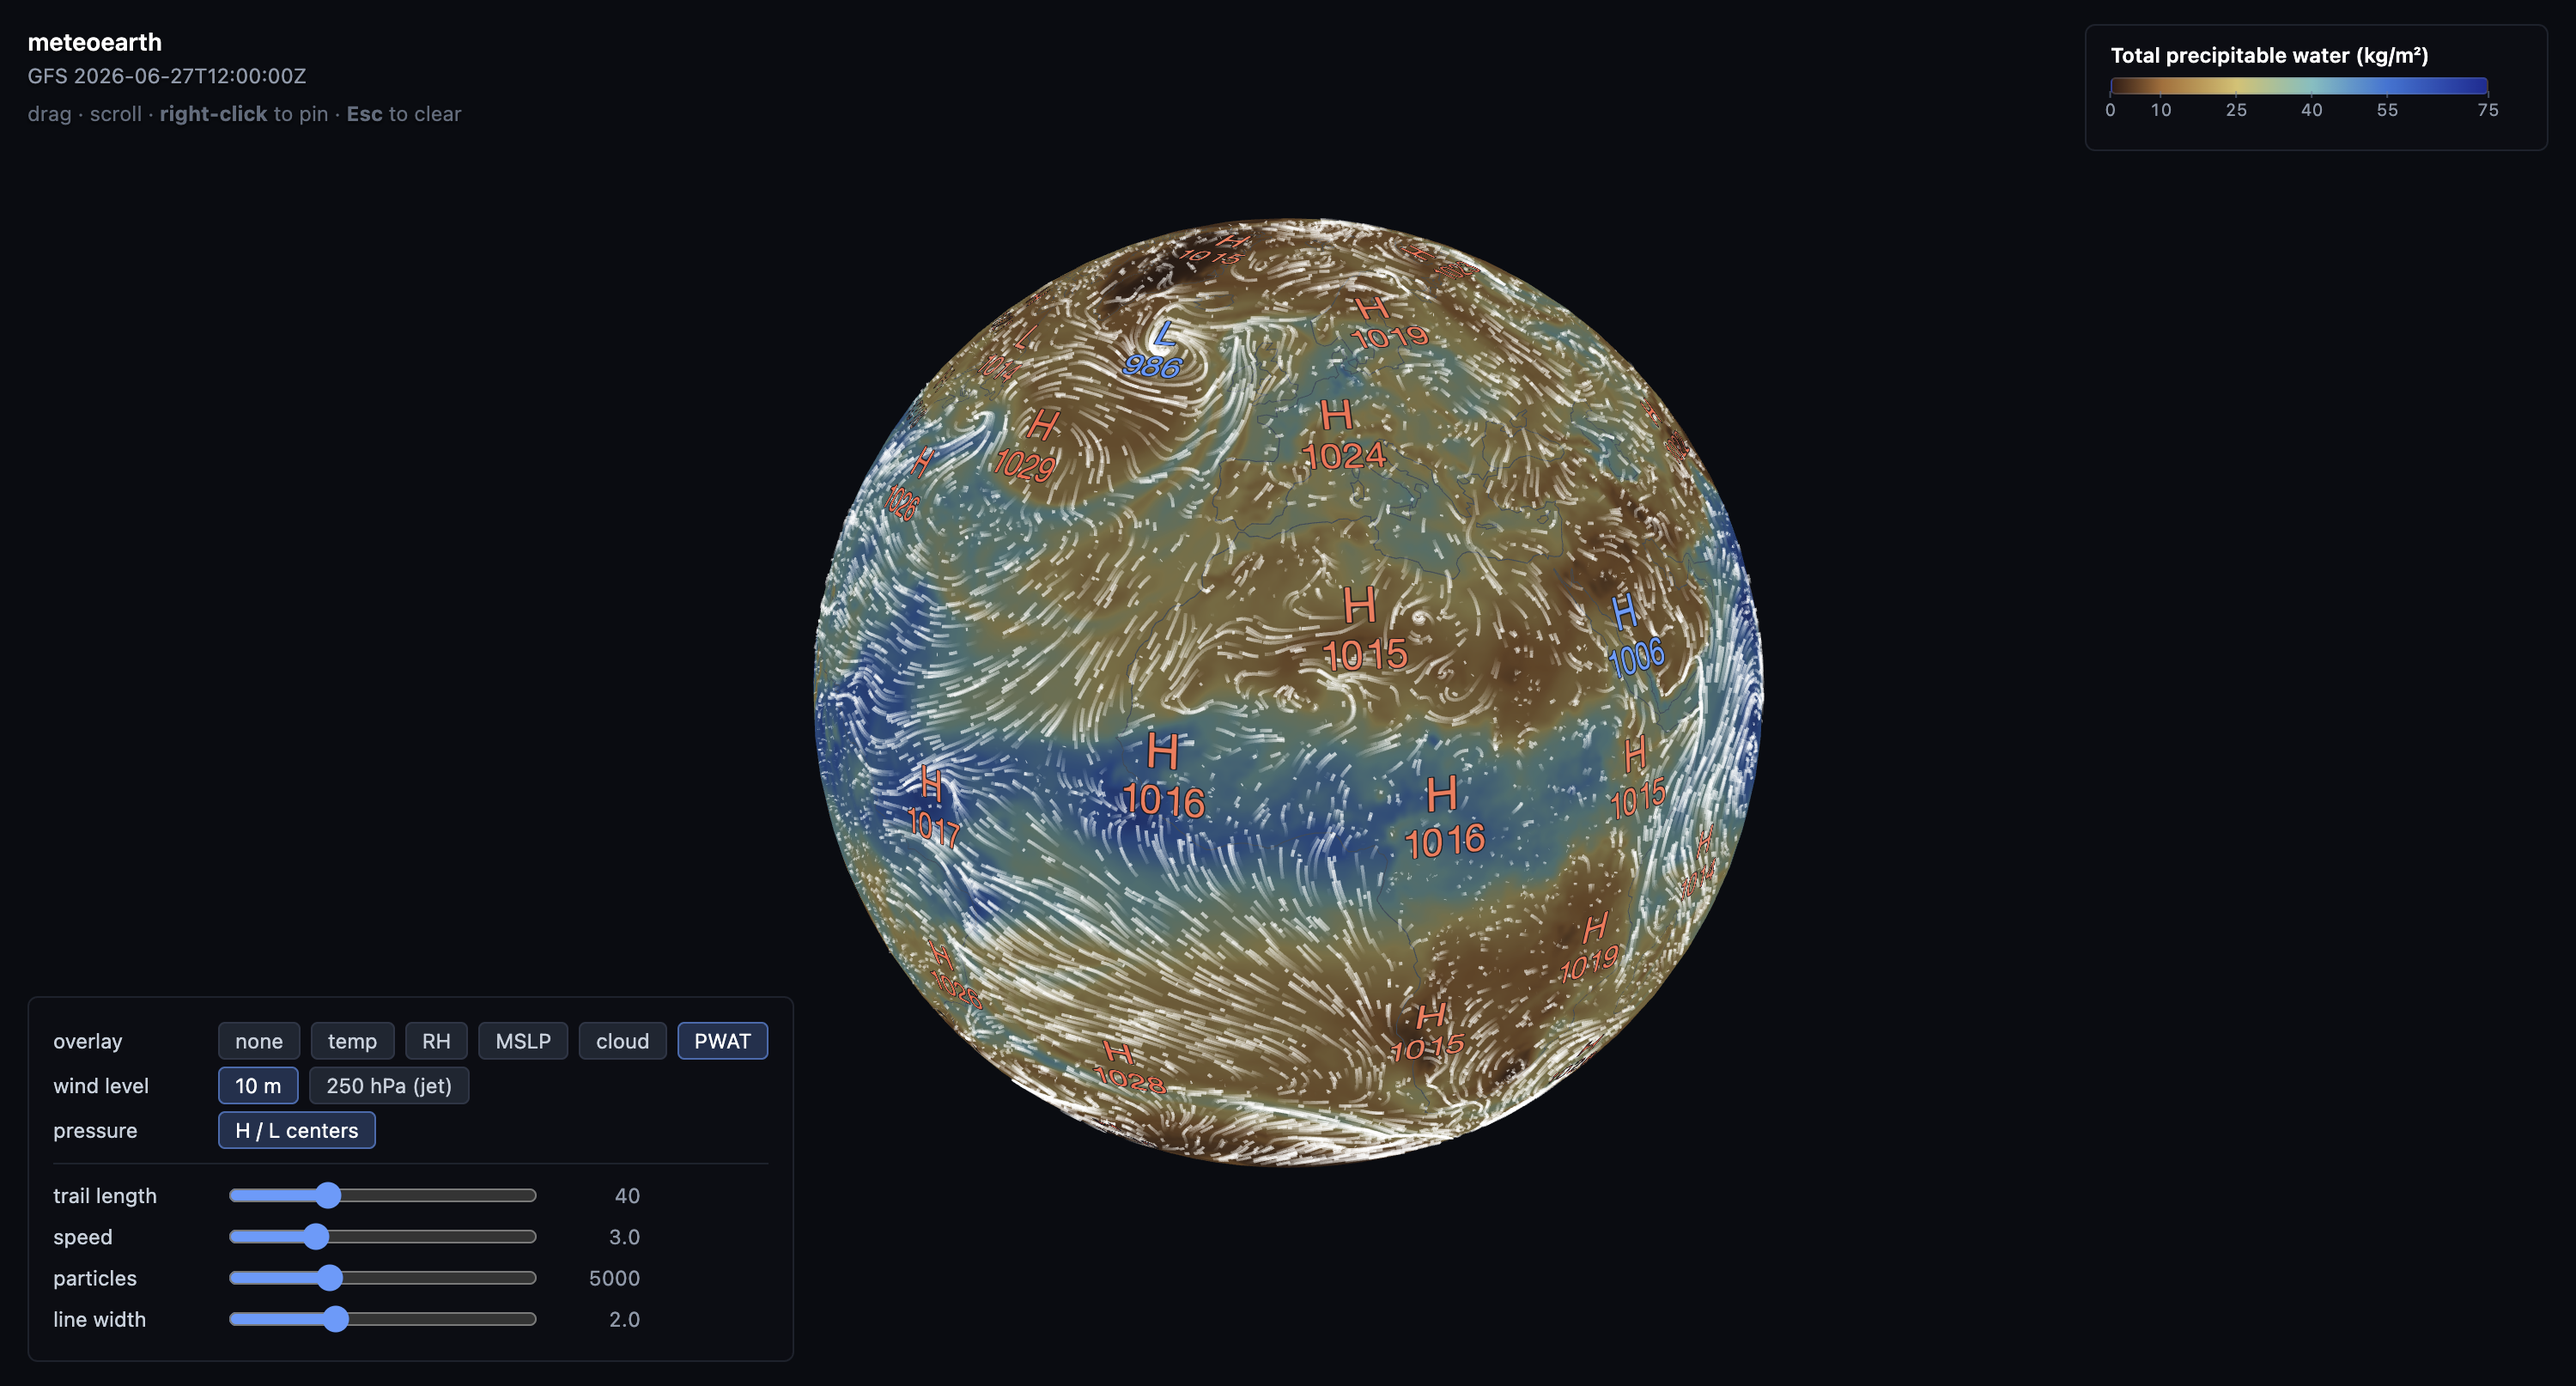
\includegraphics[width=0.92\textwidth]{fig_pwat.png}
\caption{Total precipitable water. Filaments of high column moisture
(atmospheric rivers) stand out against the dry subtropics.}
\label{fig:pwat}
\end{figure}

\section{Wind Particles and the Jet Stream}

The wind field is animated as thousands of particles advected by the vector
texture. The \textbf{wind level} buttons switch the source field between 10\,m
surface wind and 250\,hPa wind. At 250\,hPa the particles trace the jet stream
(Figure~\ref{fig:jet}): fast, coherent ribbons girdling the mid-latitudes. The
sliders tune trail length, speed, particle count, and line width in real time.

\begin{figure}[h]
\centering
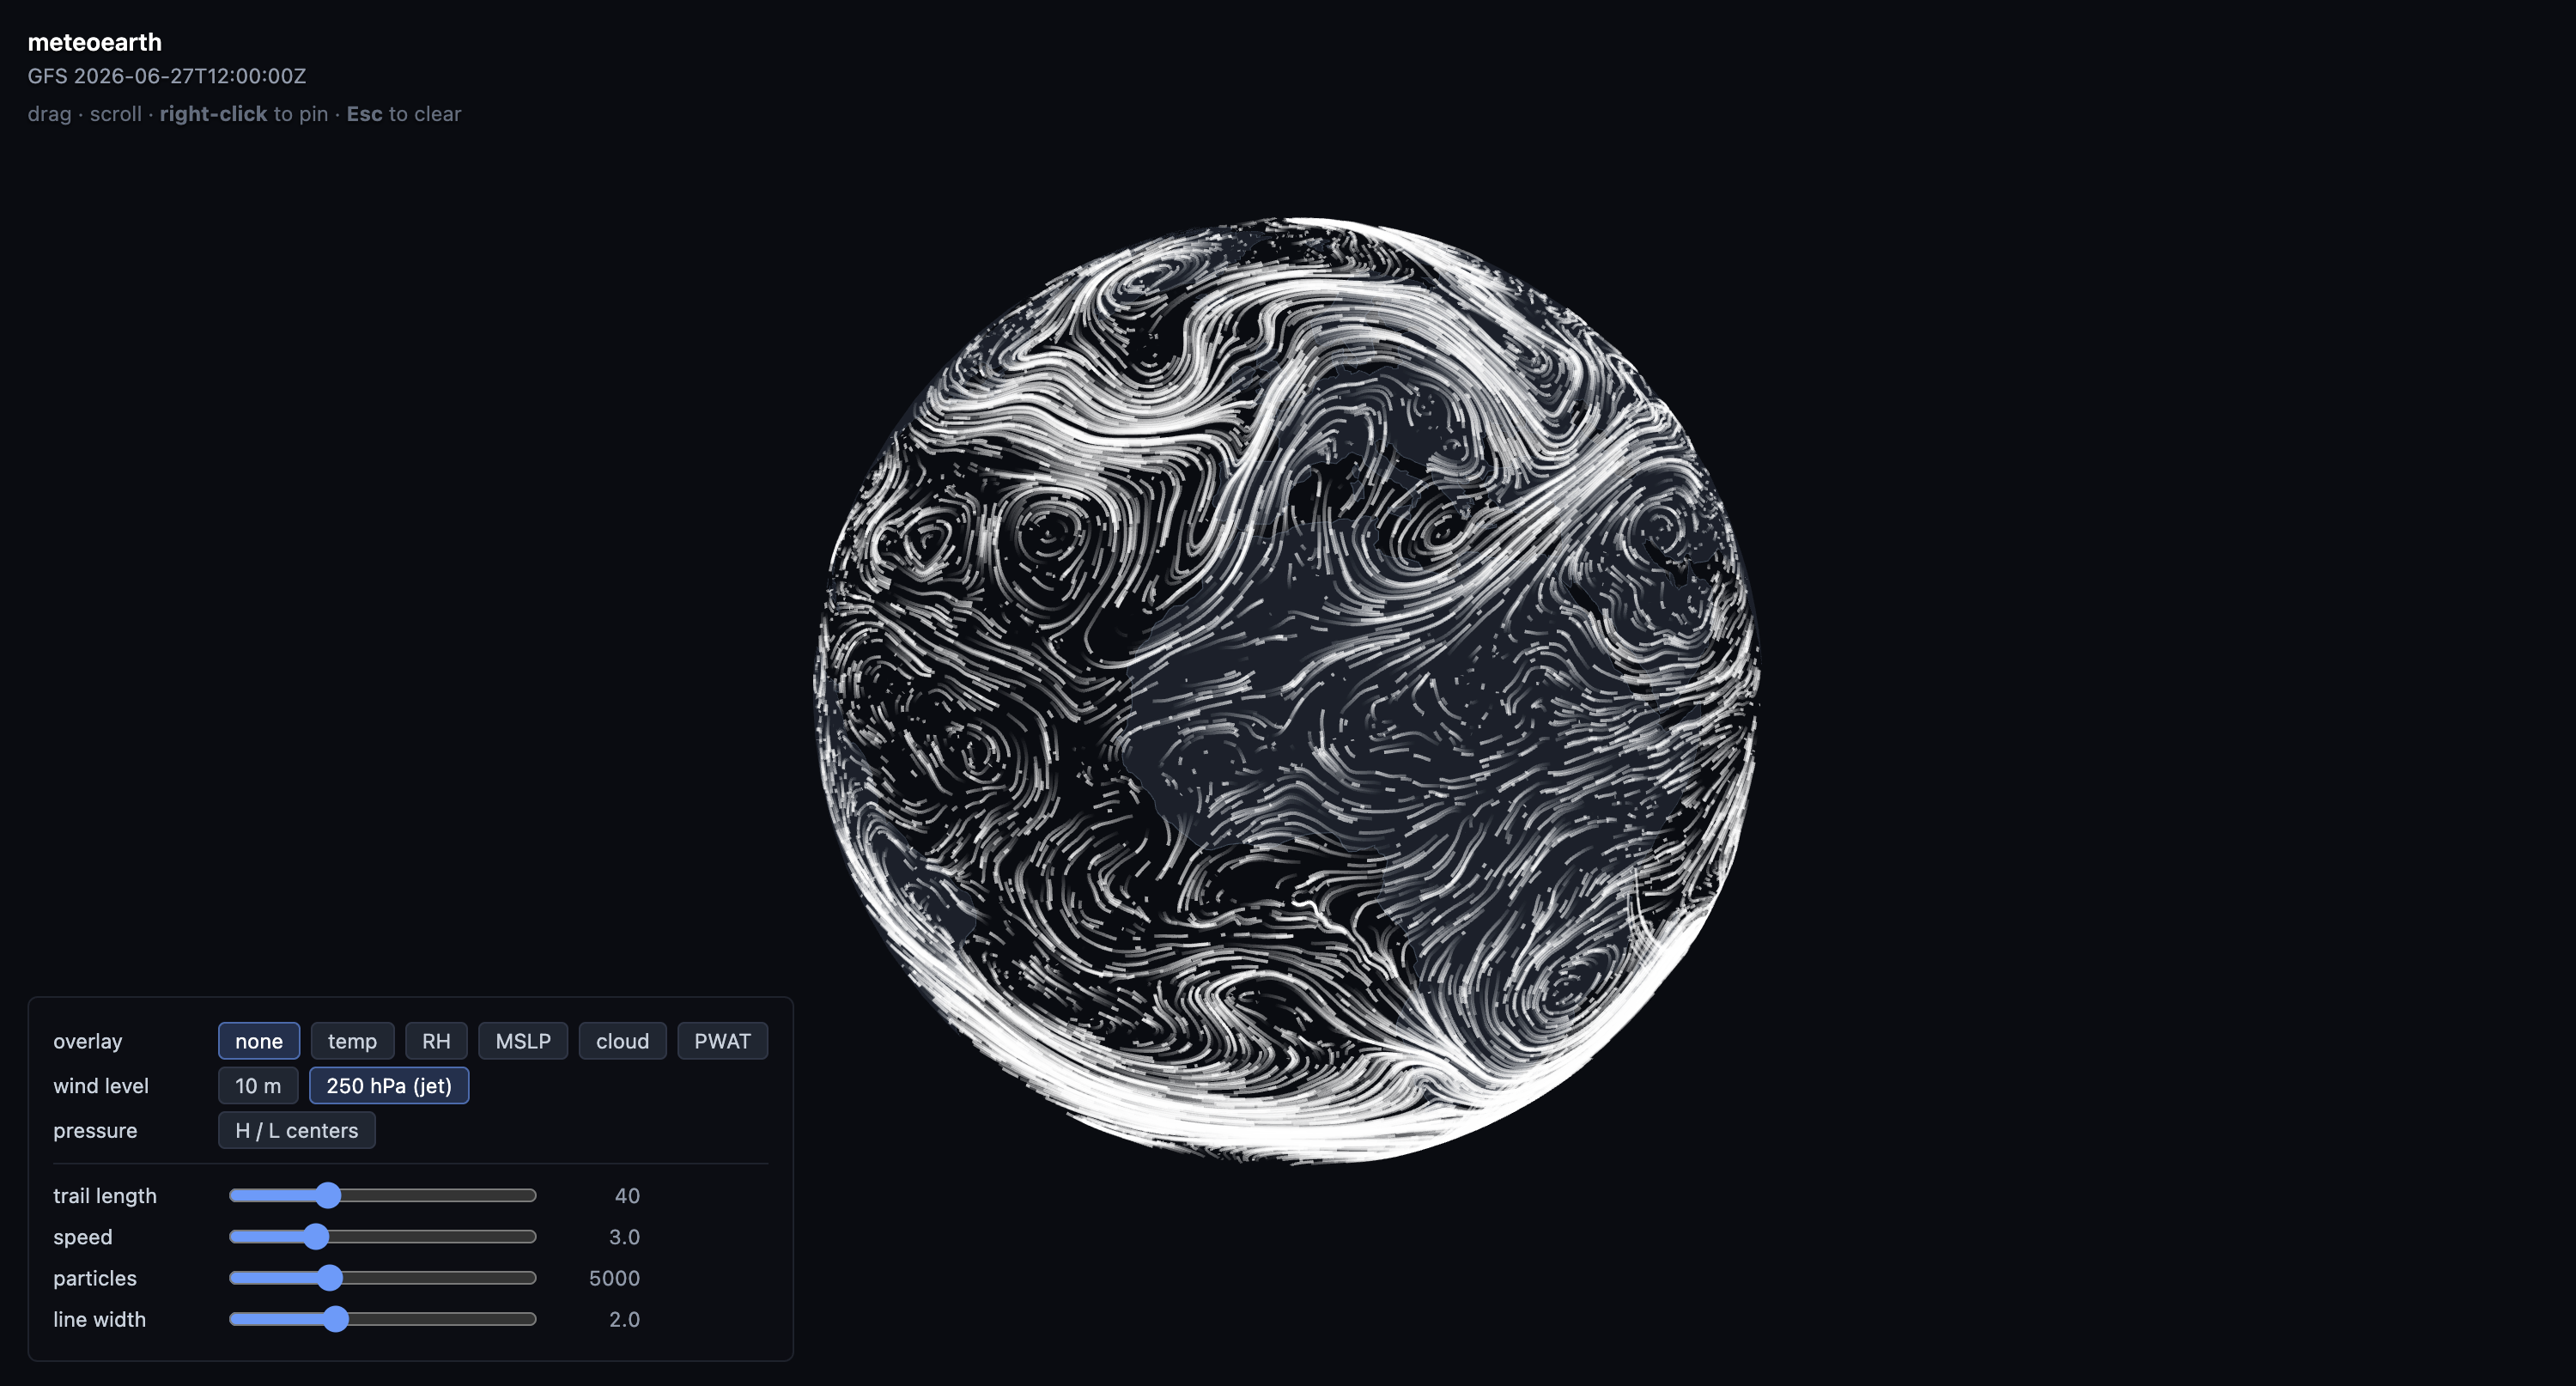
\includegraphics[width=0.92\textwidth]{fig_jet.png}
\caption{250\,hPa wind. The particle field resolves the jet stream as
high-speed, narrow ribbons, very different in character from the surface flow.}
\label{fig:jet}
\end{figure}

\section{High and Low Pressure Centers}
\label{sec:highlow}

The \texttt{H\,/\,L centers} overlay labels the eyes of the pressure systems
directly on the globe. It is computed from the mean sea-level pressure field by
WeatherLayers' \texttt{HighLowLayer}, which locates local pressure minima and
maxima and draws a large glyph at each: a blue \textbf{L} for a low-pressure
system (cyclone) and a red \textbf{H} for a high-pressure system (anticyclone),
with the central pressure printed beneath. A search radius of roughly 1500\,km
keeps the labels to the major synoptic systems rather than every minor ripple.
Figure~\ref{fig:highlow} shows the glyphs over the MSLP overlay, where each
\textbf{L} sits at the heart of a visible cyclonic vortex in the wind.

\begin{figure}[h]
\centering
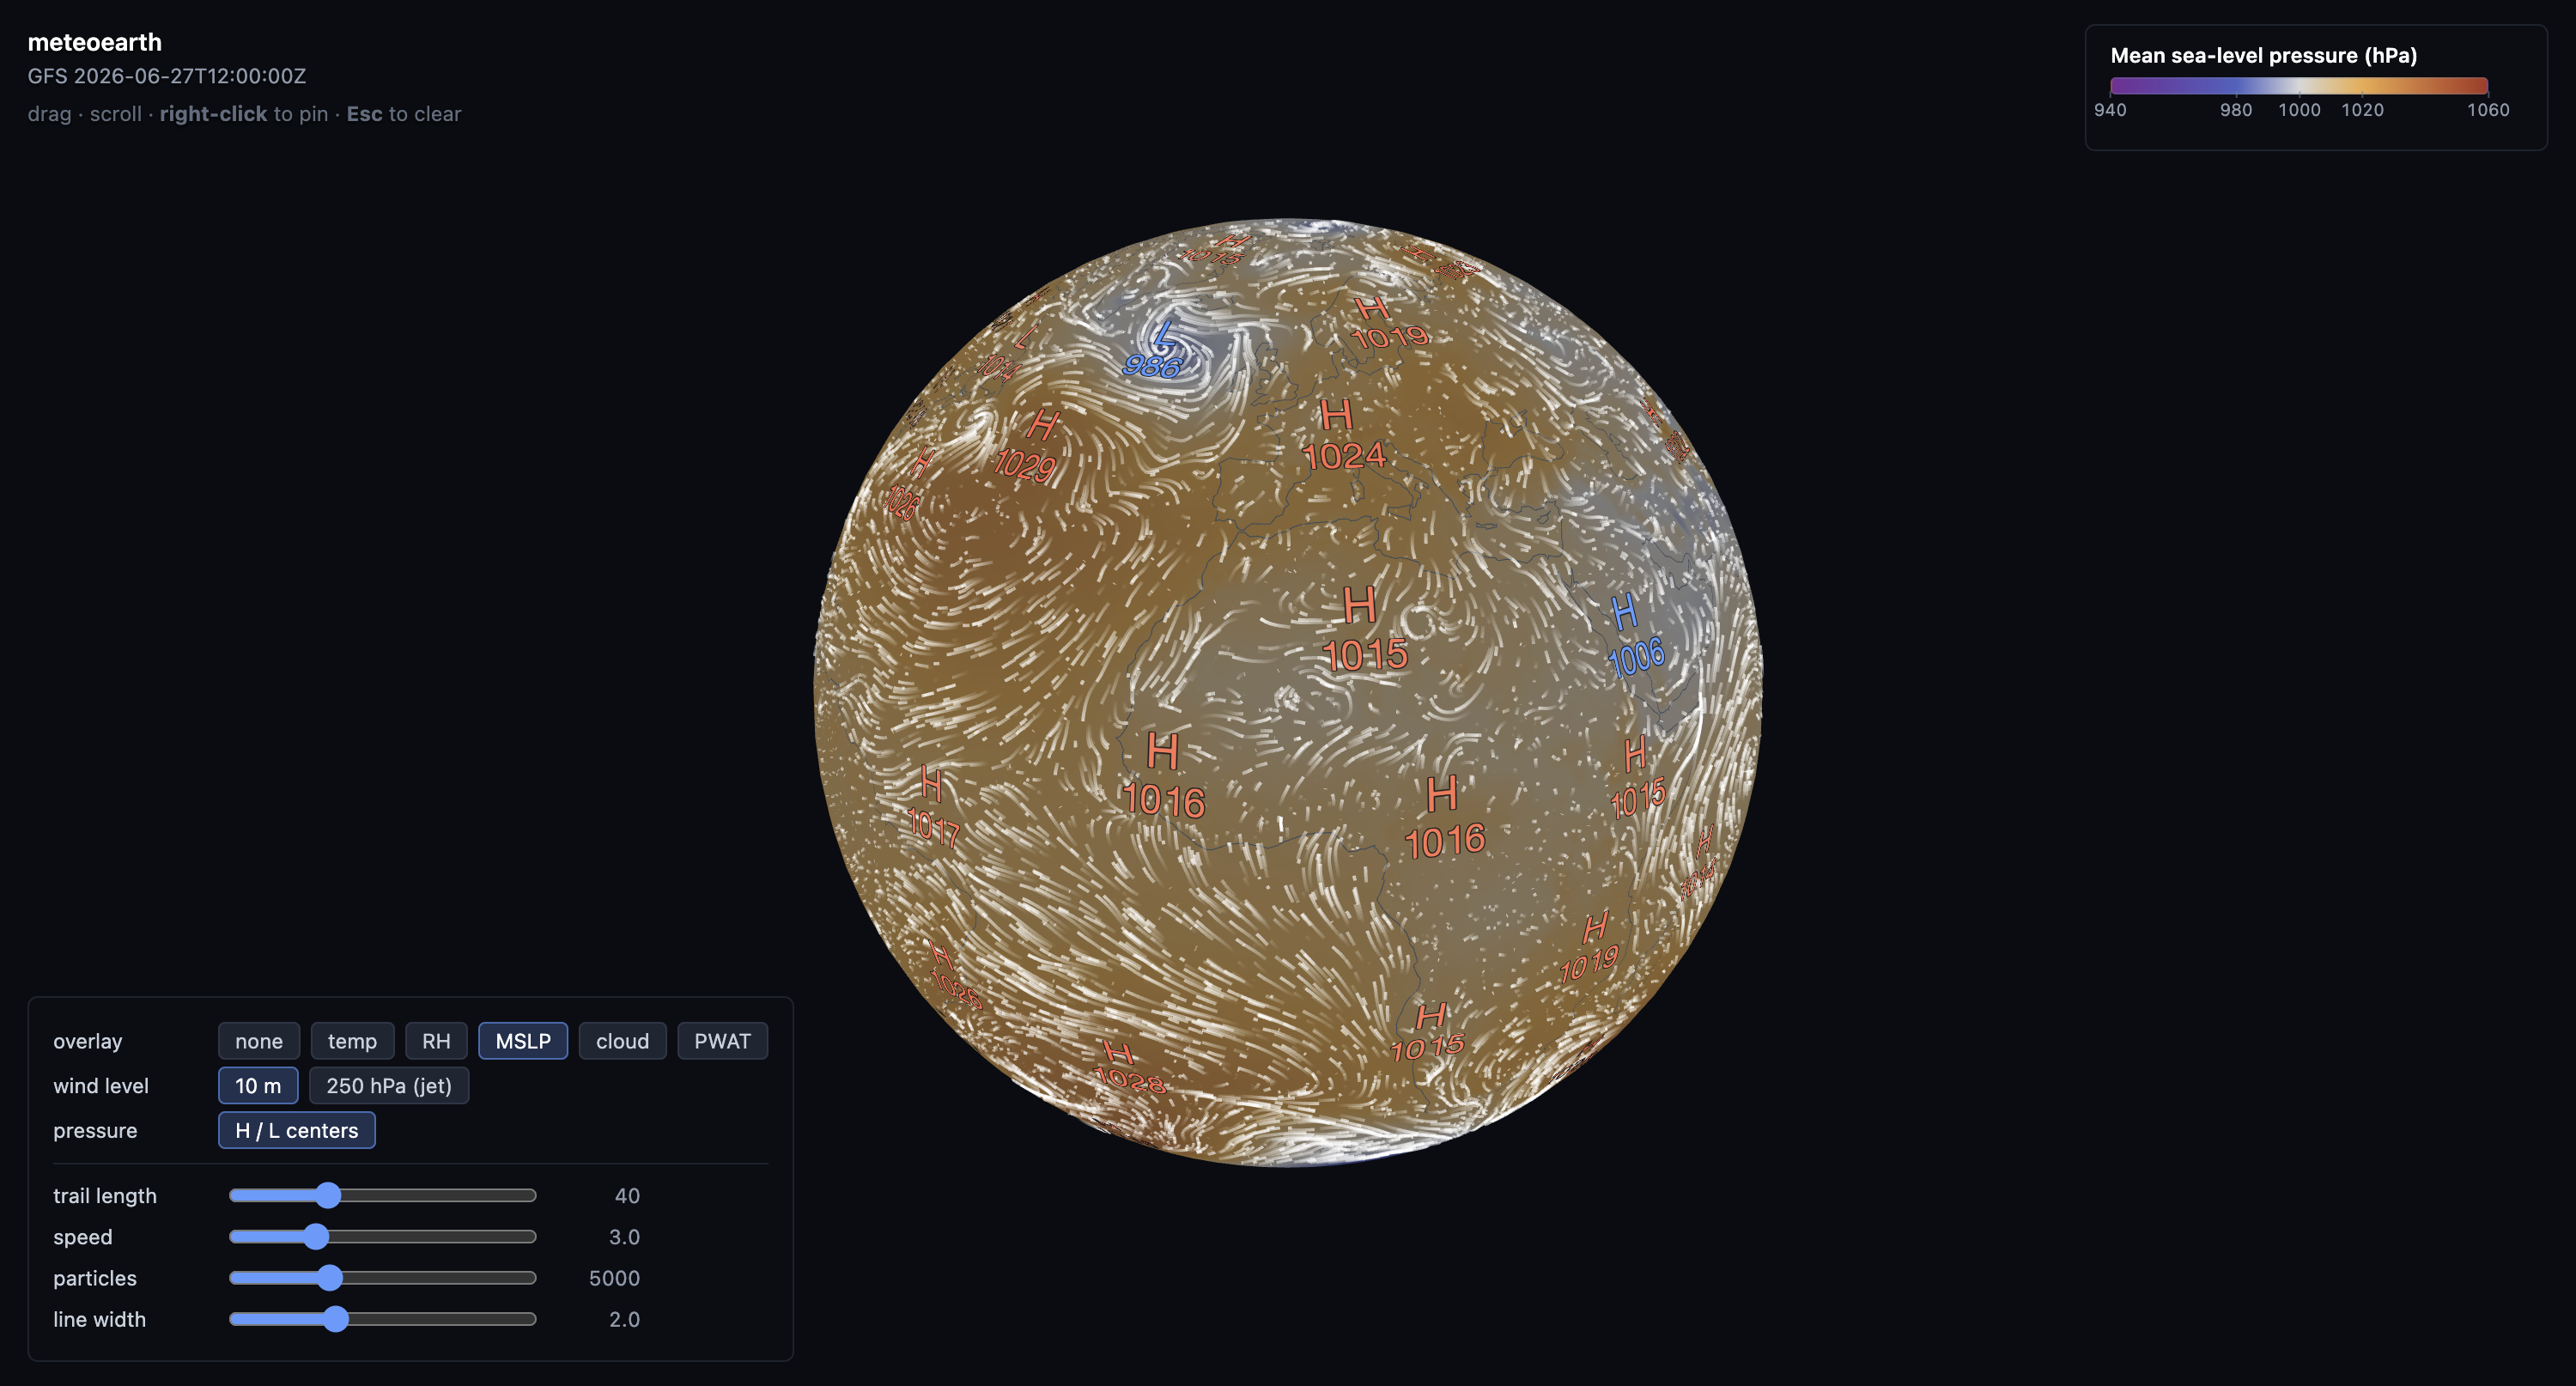
\includegraphics[width=0.92\textwidth]{fig_highlow.png}
\caption{High/low pressure centers over the MSLP overlay. Blue \textbf{L} glyphs
mark cyclones (e.g.\ the 986\,hPa low in the North Atlantic); red \textbf{H}
glyphs mark anticyclones. The central pressure is printed under each letter.}
\label{fig:highlow}
\end{figure}

Hovering a glyph replaces the point readout with a focused summary of that
system: its type, central pressure, and coordinates
(Figure~\ref{fig:highlowhover}). The glyphs ride above any active overlay, so
they can be combined with temperature, moisture, or a bare wind field. The
overlay is on by default and can be toggled off from the control panel.

\begin{figure}[h]
\centering
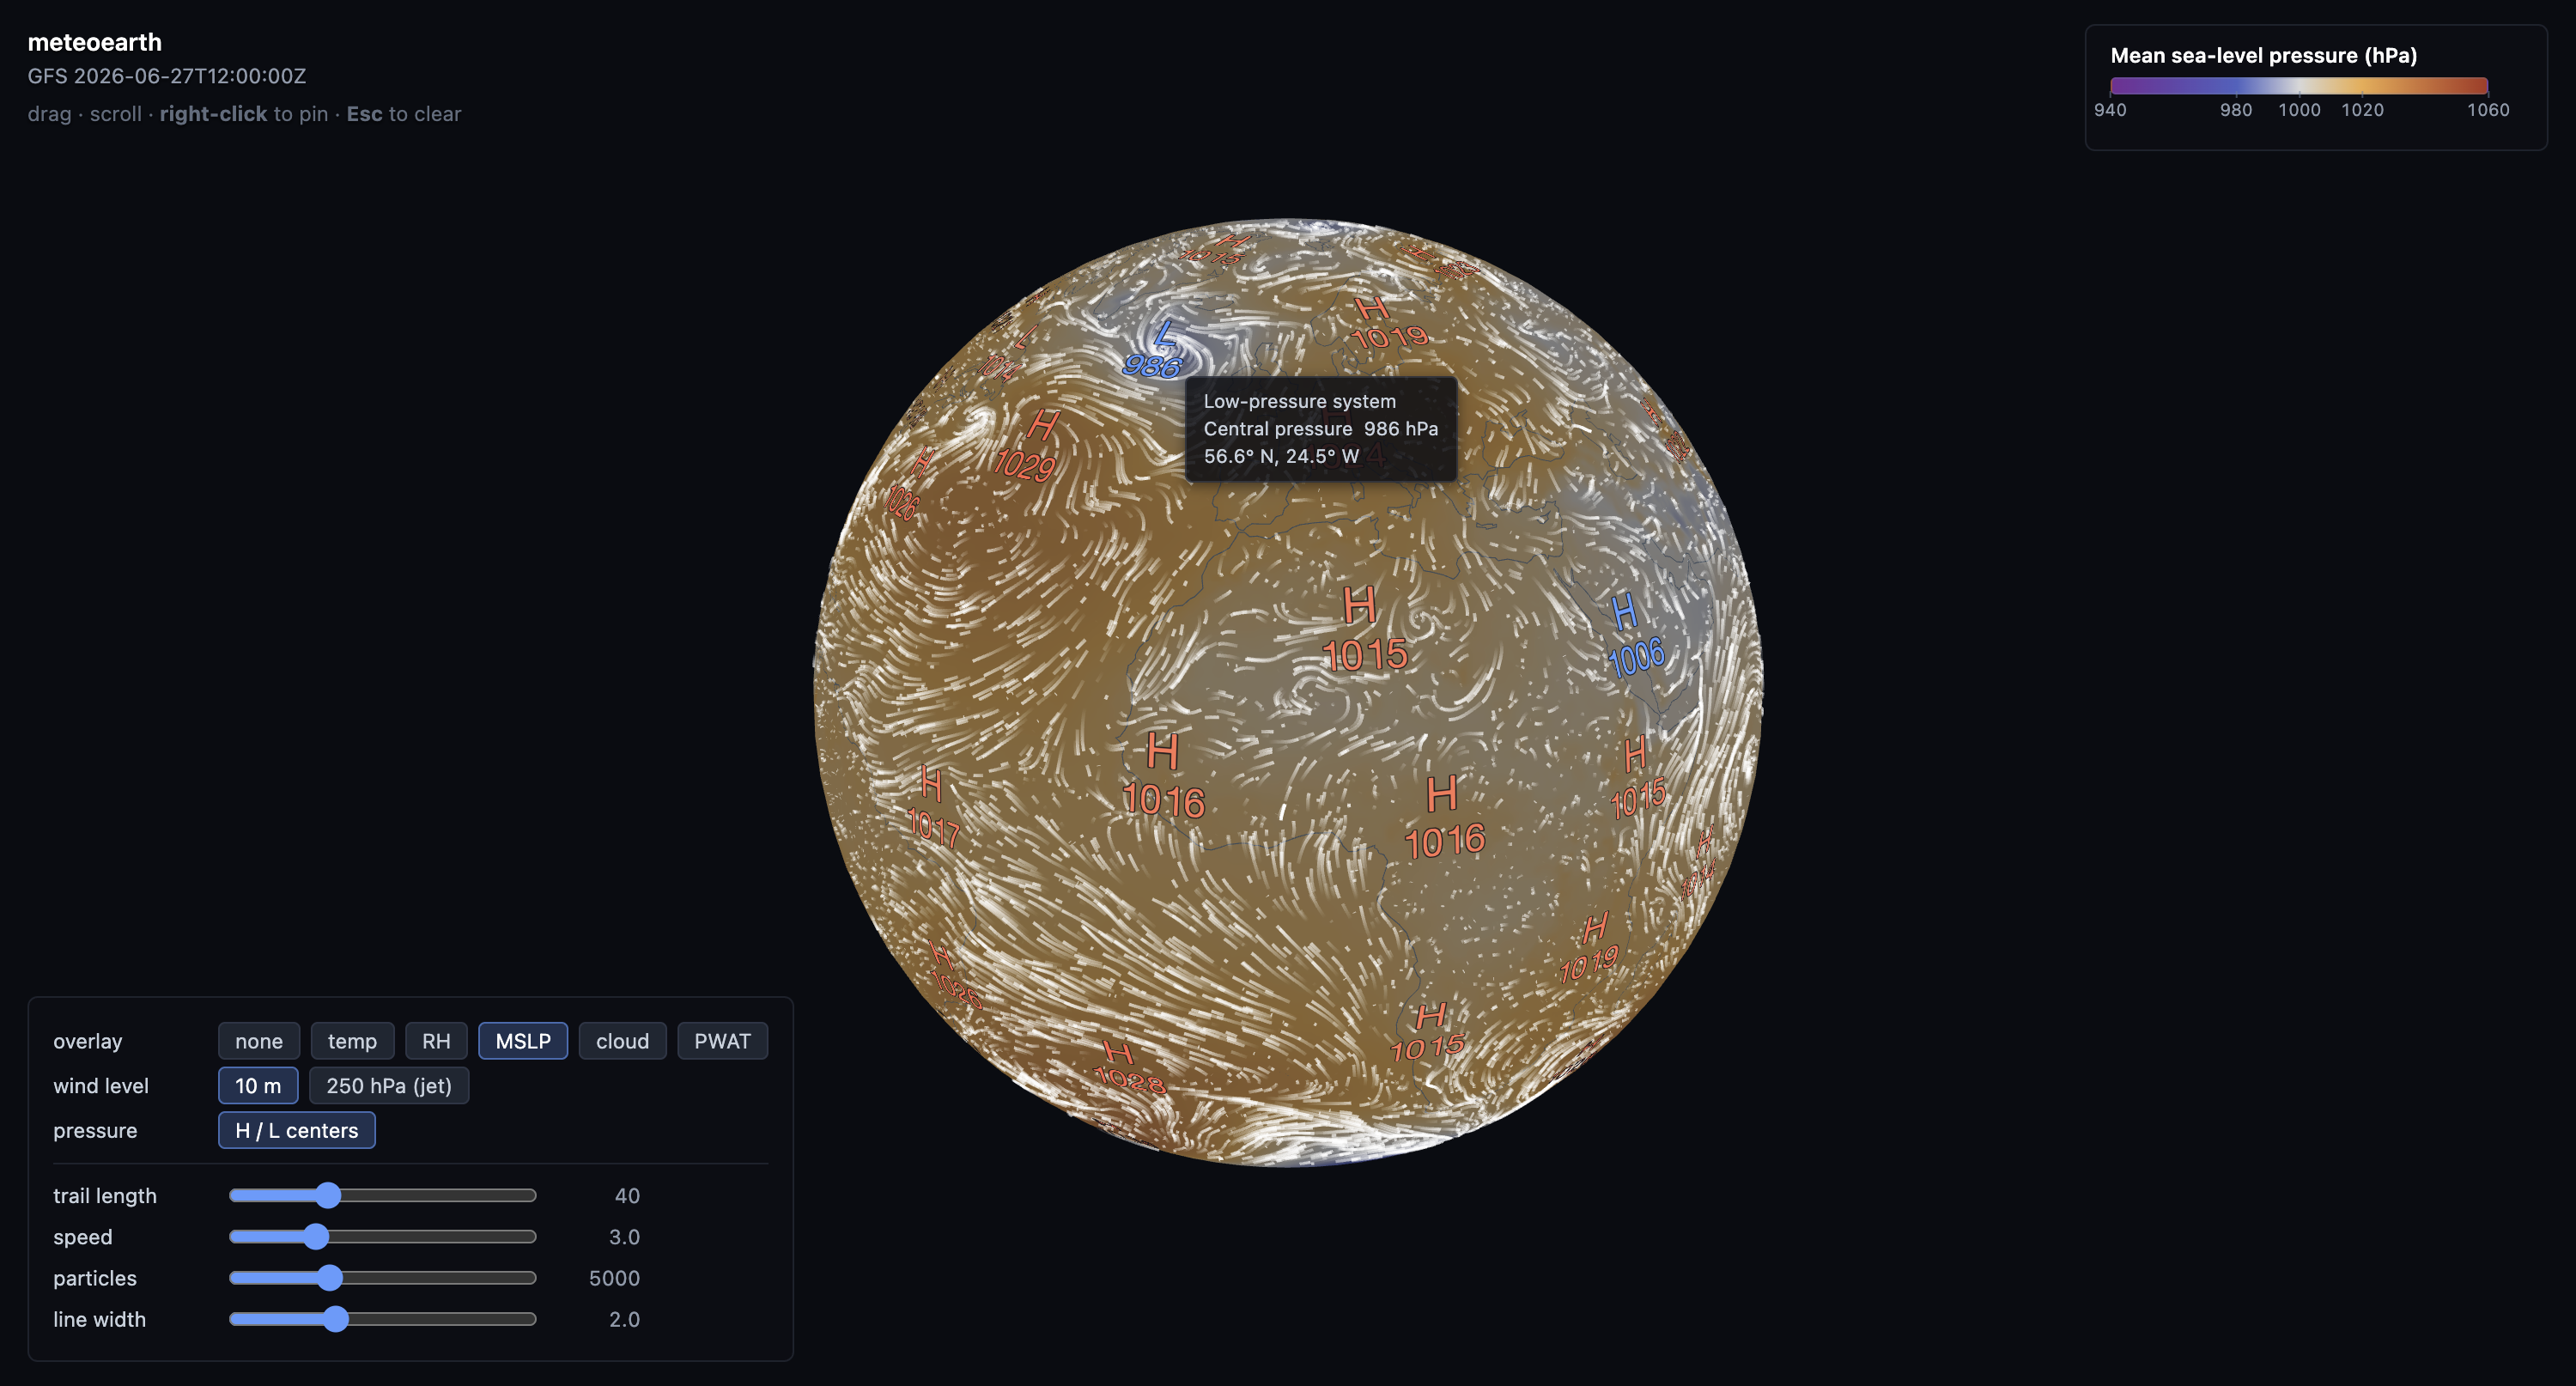
\includegraphics[width=0.92\textwidth]{fig_highlow_hover.png}
\caption{Hovering the North Atlantic low surfaces its details:
``Low-pressure system, central pressure 986\,hPa, 56.6\textdegree{}\,N,
24.5\textdegree{}\,W.''}
\label{fig:highlowhover}
\end{figure}

\section{Architecture}

\subsection{Pipeline (Python)}
\begin{itemize}
  \item \texttt{variables.py} --- the single registry of layers: NOMADS request
        parameters, cfgrib keys, unit transforms, encode ranges, and palettes.
  \item \texttt{fetch\_gfs.py} --- cycle discovery and per-variable GRIB2 subset
        download from NOMADS.
  \item \texttt{decode.py} --- GRIB2 $\rightarrow$ numpy via cfgrib, with unit
        conversion.
  \item \texttt{encode.py} --- numpy $\rightarrow$ PNG (byte-packed) plus the
        metadata JSON consumed by the frontend.
\end{itemize}

\subsection{Frontend (deck.gl + WeatherLayers)}
\texttt{frontend/src/main.js} loads every layer's PNG and JSON, then builds the
deck.gl layer stack: an invisible pickable globe polygon (so hover fires
everywhere), the optional scalar \texttt{RasterLayer}, a coastline
\texttt{GeoJsonLayer}, the WeatherLayers \texttt{ParticleLayer} for wind, the
\texttt{HighLowLayer} for pressure centers, and a pin marker. Point readouts are
computed in JavaScript by sampling the in-memory PNG bytes and un-scaling them
with each layer's \texttt{imageUnscale} range.

\section{Testing and Figures}

All screenshots and figures are produced with Selenium so they are reproducible
and never hand-captured:
\begin{itemize}
  \item \texttt{tests/auto/test\_ui.py} --- end-to-end smoke test (canvas,
        overlays, hover, pin, wind level, legend).
  \item \texttt{tests/auto/test\_highlow.py} --- verifies the pressure-center
        overlay: detection counts, glyph hover badge, toggle behavior, and that
        the point readout still carries pressure.
  \item \texttt{docs/capture\_figures.py} --- drives the app through the states
        used for the figures in this manual and writes \texttt{docs/figures/}.
  \item \texttt{docs/gen\_data\_sources.py} --- regenerates Table~\ref{tab:data}
        from the live variable registry.
\end{itemize}

The whole document, including refreshed figures and the data table, is rebuilt by
\texttt{docs/build.sh}.

\begin{thebibliography}{9}

\bibitem{gfs}
NOAA / NCEP, \emph{Global Forecast System (GFS)}.
\url{https://www.ncei.noaa.gov/products/weather-climate-models/global-forecast}

\bibitem{nomads}
NOAA NOMADS, \emph{GFS 0.5\textdegree{} GRIB filter service}.
\url{https://nomads.ncep.noaa.gov/}

\bibitem{deckgl}
deck.gl, \emph{GPU-powered, large-scale WebGL data visualization}.
\url{https://deck.gl/}

\bibitem{weatherlayers}
WeatherLayers GL, \emph{Weather visualization layers for deck.gl}.
\url{https://weatherlayers.com/}

\bibitem{cfgrib}
ECMWF, \emph{cfgrib: a Python interface to map GRIB files to xarray}.
\url{https://github.com/ecmwf/cfgrib}

\bibitem{naturalearth}
Natural Earth, \emph{Free vector and raster map data} (1:110m land).
\url{https://www.naturalearthdata.com/}

\bibitem{nullschool}
C.\ Beccario, \emph{earth :: a visual guide to global weather conditions}.
\url{https://earth.nullschool.net/}

\end{thebibliography}

\end{document}
